\section{\label{II_3_B}Proposer une interface de validation pour l'utilisateur} 

Si la redéfinition du modèle \gls{FRBR} s'effectue en \textit{backend} de l’application, par les équipes techniques et les équipes métiers du logiciel, afin de préparer l’implémentation de processus automatiques, les étapes de ces processus doivent toutefois être restituées au sein de l'interface auprès de l'utilisateur métier. Afin de donner à l'utilisateur le rôle de validation finale sur les données produites, l'espace de travail S-Movies doit permettre de visualiser les résultats afin de les valider. 

\subsection{Un enjeu de transparence}

En effet, dans le cadre de l'implémentation de fonctionnalités automatiques, fondées sur l'intelligence artificielle, la \gls{cnil} recommande que les utilisateurs soient familiarisés au fonctionnement et aux limites de ces outils, par exemple “la manière dont sont produites les sorties, les éventuels transferts de données, ainsi que les usages autorisés et les usages interdits." \footcite{zotero-item-729}. Ces informations pourraient notamment guider l’utilisateur pour la validation des données produites par les modèles. Si l'exposition de ces étapes peut être effectuée au sein de modes d'emploi dédiés, comme Skinsoft le prévoit déjà, les informations relatives aux fonctionnalités automatiques devront toutefois être directement intégrées à l’interface pour un souci de transparence. Ainsi, la \gls{cnil} recommande que "l’intégration de briques d’IA générative dans un système d’information (SI) devrait être pensée avec des éléments de design informant clairement les utilisateurs de l’origine de la proposition [...]." \footcite{zotero-item-729}.
De plus, en cas de non-validation des données produites par l'utilisateur, il pourrait être pertinent de proposer "un point de contact pour remonter des problèmes ou des difficultés d’ordre éthique"\footcite{zotero-item-729}. L’interface devra ainsi prévoir un formulaire décrivant la raison du refus des données, envoyé à l’équipe technique afin que l'algorithme puisse être amélioré, voire affiné. Au cours de notre stage, un système similaire a été proposé afin de prévoir la gestion des erreurs d'un outil de recherche en langage naturel, visible en Annexe B (\ref{annexe_B}). Un formulaire est prévu pour l'utilisateur en cas de résultats non pertinents pour que le processus soit amélioré.

\subsection{Développer une interface dédiée à la validation de l'utilisateur}
Si notre étude ne relève pas de l'\gls{ia} générative, il est toutefois pertinent d'offrir à l'utilisateur un niveau de transparence maximal au sein de l'interface, via la viualisation des données produites et leur validation finale. À l'image des deux phases de traitement automatiques développées dans les sections précédentes (segmentation et classification), la validation côté interface pourra prendre la forme de deux phases de décision. Il pourra d'abord être demandé à l'utilisateur d'actionner ou non le processus de segmentation puis de le valider ou de l'invalider. Une fois le processus de segmentation finalisé, l'utilisateur pourra décider de déclencher le processus de détection d'objets sur les segments produits, puis de finalement les modifier ou de les valider.
Afin de concrétiser le processus de validation côté interface, nous nous appuyons sur l'exemple de la plateforme Amalia.js, développée par l'\gls{ina} en 2015, conçue pour visualiser les résultats d’algorithmes d’analyse audiovisuelle \footcite{zotero-item-740}. Le besoin à l'origine d'Amalia.js est donc de permettre de visualiser les résultats divers issus de pipelines d'automatisation \footcite{herve2015}. Cette interface permettrait d'une part de visualiser les résultats et d'autre part, de vérifier la conformité des données produites en lien avec les standards métiers en vigueur au sein du logiciel \footcite{herve2015}. L'interface permet également d’annoter directement le flux vidéo afin de corriger les données produites \footcite{herve2015}. La correction effectuée par l'utilisateur  permet de constituer des données d'entraînement supplémentaires afin d'améliorer les algorithmes d'indexation automatique \footcite{herve2015}. 
Amalia.js intègre notamment un \textit{plugin} de \textit{timeline} pour l'affichage des segments temporels et des images-clés associées, ainsi qu'un \textit{plugin} de superposition (\textit{overlay}) qui permettrait l'affichage de l'encadrement des objets détectés \footcite{zotero-item-740}.
Plutôt que de développer deux modules distincts, cette logique pourrait être combinée au sein de S-Movies sous la forme d'un module d'édition des données. Ce module présenterait d'abord à l'utilisateur la ligne temporelle des séquences associées aux images-clés, puis après leur validation, le module prévoierait l'ouverture d'une fenêtre d'édition latérale contenant les propositions de mots-clés et les objets détectés entourés au sein des images-clés. Ce module d'édition s'inspire du \textit{plugin} \textit{Editor} au sein d'Amalia.js dont la figure \ref{figamalia} ci-dessous ilustre la disposition : 

\begin{figure}[H] 
	
	\centering 
	
	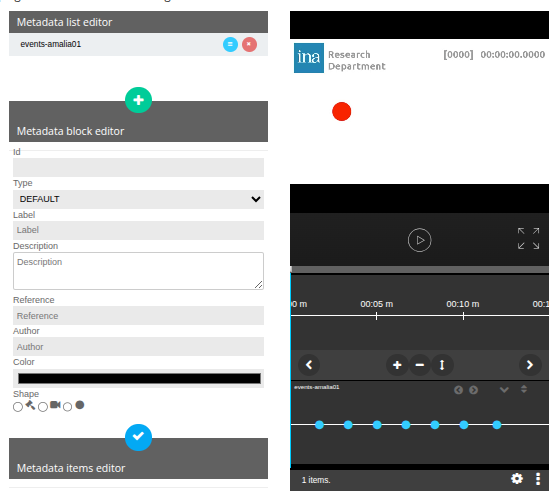
\includegraphics[width=1.0\textwidth]{images/amalia.png} 
	
	\caption{\textit{Plugin Editor} dans Amalia.js \footcite{zotero-item-794}} 
	
	\label{figamalia} 
	
\end{figure}

En cas de modification par l'utilisateur, l'interface pourrait enregistrer les données validées, tout en les envoyant en \textit{backend}, afin que le processus soit amélioré. 
Le développement de l'interface serait ainsi conforme à la mise en place d'une automatisation facilitatrice de la création de données, en incitant l'utilisateur "à vérifier les données fournies en entrée et la qualité des sorties" \footcite{zotero-item-729}.

\subsection{Déroulé du processus de validation}

Concrètement, en \textit{frontend}, dans l’interface de l’application prévue pour l’utilisateur, le processus suivant peut-être imaginé, illustré par un diagramme de décision (\ref{fig:validation}):

\begin{figure}[H] 
	
	\centering 
	
	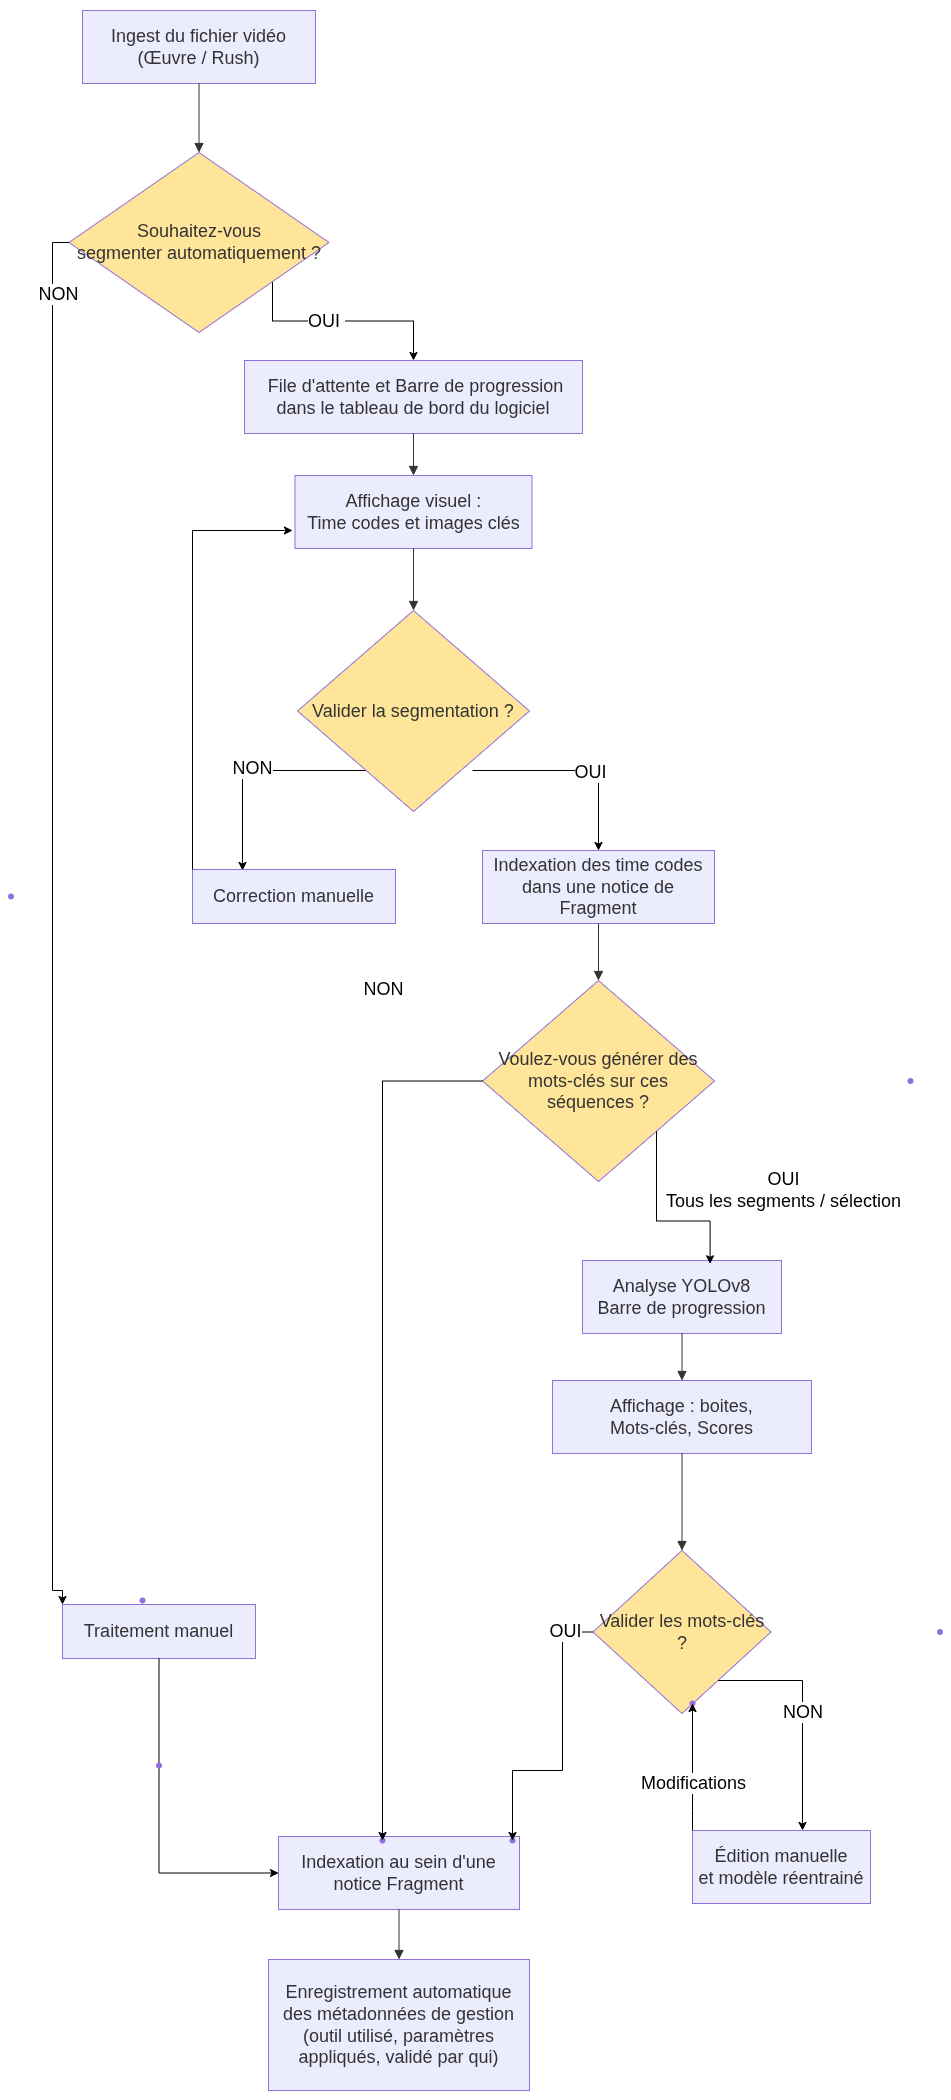
\includegraphics[width=0.6\textwidth]{images/validation.png} 
	
	\caption{Processus de validation de l'utilisateur métier} 
	
	\label{fig:validation} 
	
\end{figure}

Ce processus permet de laisser l'utilisateur métier décider de l'indexation des données via l'actionnage ou non des fonctionnalités automatiques. L'utilisateur décide en amont du processus, et valide ensuite les données produites à es fins d'indexation. 

%Exemple de la plateforme okapi :  

%“Okapi fournit un ensemble d’outils destiné à l’analyse sémantique et sémiotique de contenus multimédia (vidéo, image, son) et à la gestion de corpus de vidéos, d’extraits sonores et de parties d’images. Les outils d’analyse permettent l’indexation et la description sémantique de contenu sur la base d’ontologies qui décrivent les objets et classes des domaines étudiés. Les outils de gestion de corpus fournissent des services pour la constitution, la visualisation, l’enrichissement et la valorisation de corpus thématiques.” \footcite{lalande2022} (cf capture d'écran)